\placelogofalse
\begin{frame}{Adaptive Partition Scanning (APS)}
\begin{columns}
\column{0.48\linewidth}
\centering
\begin{outline}
  \1 Dynamically decide \# of partitions to scan
  \1 Geometric Model Assumptions
  \2 $\rho_k = $ Distance to  $k$-th nearest neighbor
  \2 Uniform Density in query Hypersphere
  \2 Partition = half space
  \2 Partition intersection is sphere cap
\end{outline}

$$
\text{Recall}_i = \frac{\text{Vol}\left(B(q, \rho_k) \cap P_i\right)}{\text{Vol}\left(B(q, \rho_k) \right)}
$$

\column{0.48\linewidth}
\begin{center}
\centering
\begin{align*}
  p_0 &= \prod_{j=1}^{M - 1} (1 - v_j)\\
  p_i &= (1 - p_0)v_i
\end{align*}

\vspace{0.2cm}

%\shadowimage[width=2.5cm]{example_1.png}

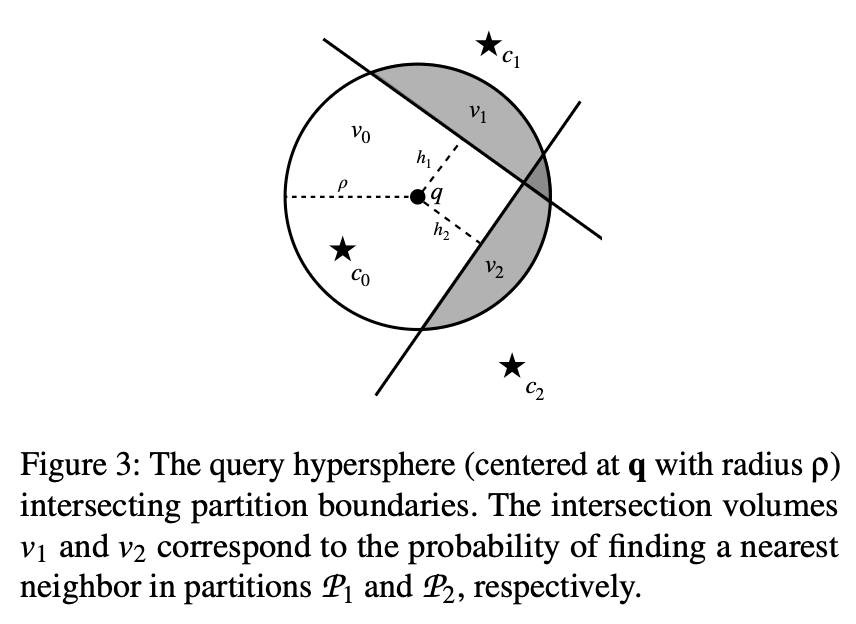
\includegraphics[width=5.0cm]{assets/fig_3.png}

% [trim={left bottom right top},clip]
%\includegraphics[width=8.5cm, page=3, trim={0 9cm 14cm 0cm},clip]{assets/vec_db_figs.pdf}
\end{center}
\end{columns}
\end{frame}
\placelogotrue
